% Experiments Section
% This file contains the experimental results

\section{Experiments}
\label{sec:experiments}

We conduct comprehensive experiments to validate the effectiveness of Spiral RoPE across multiple vision tasks: image classification on ImageNet-1k, semantic segmentation on ADE20k, and class-conditional image generation on ImageNet. Our experiments demonstrate that Spiral RoPE consistently improves performance over baselines and prior 2D RoPE methods.

\subsection{Image Classification}
\label{sec:experiments:classification}

\paragraph{Setup.} We evaluate Spiral RoPE on ImageNet-1k \cite{dengImageNetLargescaleHierarchical2009} classification using DeiT \cite{touvronTrainingDataefficientImage2021} as the base architecture. We train DeiT-Small, DeiT-Base and DeiT-Large models with and without Spiral RoPE on three target resolutions: $224 \times 224$, $384 \times 384$, and $448 \times 448$. Following \cite{heoRotaryPositionEmbedding2024}, we combine Spiral RoPE with the original absolute positional embedding (APE), as this combination has been shown to be effective. We use $K=16$ directions for Spiral RoPE with all frequencies $\theta_t$ scaled by a factor of 1.5 (i.e., $\theta_t = 1.5\theta_{\text{base}}^{-t/(d/4)}$). Models are pre-trained at $224 \times 224$ resolution for 300 epochs (Small and Base) or 200 epochs (Large), then fine-tuned at the target resolution for 20 epochs. We compare against the standard DeiT baseline and RoPE-Mixed \cite{heoRotaryPositionEmbedding2024}, which uses learnable per-head frequencies, in contrast to our method that uses pre-specified directions and frequencies. For evaluation, we report Top-1 accuracy on the validation set using the final checkpoint with exponential moving average (EMA) weights and full crop (crop ratio = 1.0). Additional training details are provided in Appendix~\ref{app:details}.

\paragraph{Results.} \cref{tab:classification} presents the classification results across different resolutions. Spiral RoPE consistently outperforms both the APE baseline and RoPE-Mixed across all configurations. These results demonstrate that the multi-directional encoding in Spiral RoPE provides richer positional information that benefits image classification, with larger improvements observed at higher resolutions.

\begin{table}[t]
    \caption{\textbf{\textit{ImageNet-1k classification accuracy (\%).}} Models are pre-trained at $224 \times 224$ and fine-tuned at each target resolution. Spiral RoPE consistently outperforms baselines across all configurations.}
    \label{tab:classification}
    \begin{center}
        \begin{small}
            \begin{sc}
                \begin{tabular}{llccc}
                    \toprule
                    Model & Method & 224 & 384 & 448 \\
                    \midrule
                    \multirow{3}{*}{DeiT-S} 
                    & APE & 79.11 & 81.88 & 82.24 \\
                    & RoPE-Mixed & \textbf{80.48} & 82.64 & 82.99 \\
                    & Spiral RoPE (ours) & 80.39 & \textbf{83.04} & \textbf{83.15} \\
                    \midrule
                    \multirow{3}{*}{DeiT-B} 
                    & APE & 82.36 & 84.16 & 84.29 \\
                    & RoPE-Mixed & 83.15 & 84.73 & 84.84 \\
                    & Spiral RoPE (ours) & \textbf{83.39} & \textbf{85.04} & \textbf{85.19} \\
                    \midrule
                    \multirow{3}{*}{DeiT-L} 
                    & APE & 83.24 & 84.92 & 85.13 \\
                    & RoPE-Mixed & 83.51 & 85.14 & 85.40 \\
                    & Spiral RoPE (ours) & \textbf{83.97} & \textbf{85.48} & \textbf{85.67} \\
                    \bottomrule
                \end{tabular}
            \end{sc}
        \end{small}
    \end{center}
    \vskip -0.1in
\end{table}

\paragraph{Extrapolation Robustness.} We further evaluate robustness to input resolutions unseen during training. Using models trained and fine-tuned at $224 \times 224$ resolution, we evaluate performance across resolutions ranging from $144 \times 144$ to $512 \times 512$. Other evaluation settings are the same as before. For resolution extrapolation, APE employs bicubic interpolation to resize the learned position vectors from training to evaluation resolution. RoPE-based methods extend position indices to the new grid size while preserving the same frequency patterns, enabling smooth extrapolation through the inherent continuity of trigonometric functions.

\cref{fig:multires} shows the extrapolation robustness results for both DeiT-Base and DeiT-Large models. Both Spiral RoPE and RoPE-Mixed consistently outperform APE across all resolutions and model sizes, demonstrating the advantage of rotary position embeddings for resolution generalization. At lower resolutions near the training resolution, Spiral RoPE and RoPE-Mixed perform comparably. However, at higher resolutions (\emph{e.g.}, $384 \times 384$ to $512 \times 512$), our Spiral RoPE exhibits a clear advantage over RoPE-Mixed across both model sizes, suggesting that our method with pre-specified directions and fixed sinusoidal frequencies achieves better extrapolation than RoPE-Mixed with learned frequencies when evaluating on unseen resolutions.

\begin{figure}[t]
    \centering
    \begin{subfigure}[b]{0.9\columnwidth}
        \centering
        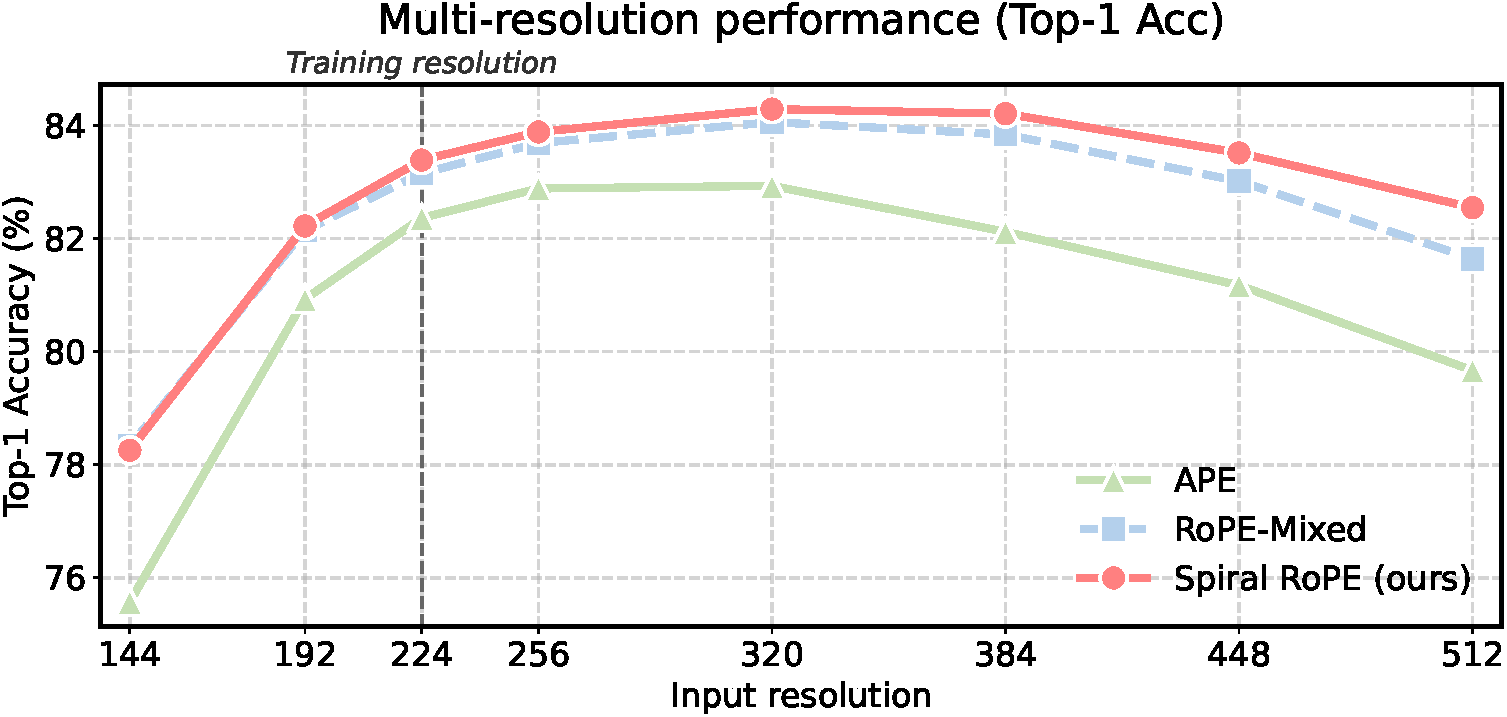
\includegraphics[width=\linewidth]{plots/multires_robustness_base.pdf}
        \caption{DeiT-Base}
    \end{subfigure}
    \\[0.3em]
    \begin{subfigure}[b]{0.9\columnwidth}
        \centering
        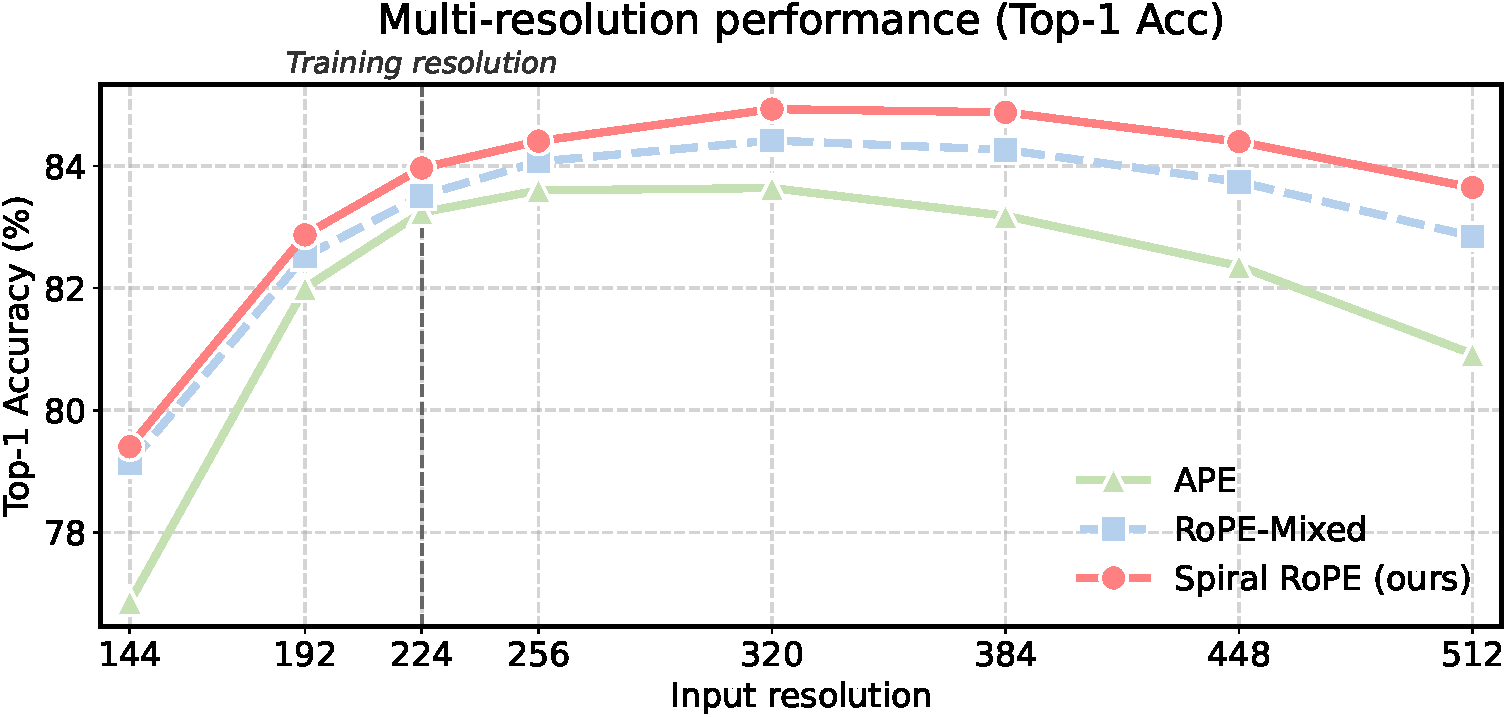
\includegraphics[width=\linewidth]{plots/multires_robustness_large.pdf}
        \caption{DeiT-Large}
    \end{subfigure}
    \caption{\textbf{\textit{Multi-resolution performance on ImageNet-1k}}. Models are trained at $224 \times 224$ and evaluated across resolutions from $144 \times 144$ to $512 \times 512$. Spiral RoPE demonstrates superior robustness to resolution changes compared to APE and RoPE-Mixed baselines across both model sizes.}
    \label{fig:multires}
\end{figure}

\subsection{Semantic Segmentation}
\label{sec:experiments:segmentation}

\paragraph{Setup.} We evaluate Spiral RoPE on semantic segmentation using the ADE20k dataset \cite{zhouSceneParsingADE20K2017a, zhouSemanticUnderstandingScenes2018a}, which contains 20,000 training images and 2,000 validation images across 150 semantic categories. We use UperNet \cite{xiaoUnifiedPerceptualParsing2018} as the segmentation framework with ViT training recipe, and we initialize the backbone with the ImageNet pre-trained weights at $224 \times 224$. The segmentation models are trained at $512 \times 512$ resolution for 160k iterations with a batch size of 16. For evaluation, we perform single-scale testing on the validation set and report mean Intersection over Union (mIoU), mean class accuracy (mAcc), and overall pixel accuracy (aAcc). Additional training details are provided in Appendix~\ref{app:details}.

\paragraph{Results.} \cref{tab:segmentation} summarizes semantic segmentation results on ADE20k, where Spiral RoPE consistently achieves significant improvements over the original APE baselines. Remarkably, we observe that the DeiT-Large model attains a notable mIoU of 49.12\%, substantially outperforming the original baseline of 46.91\% at virtually no additional computational cost. Moreover, the gains brought by Spiral RoPE on the ADE20K semantic segmentation task are intuitively more pronounced than those observed in classification (\emph{e.g.}, 3.06\% vs. 0.73\% accuracy improvement), suggesting that for dense prediction tasks such as semantic segmentation where reasoning is more complex and higher input resolutions are required, a well-designed relative position embedding can more effectively facilitate the modeling of spatial dependencies, demonstrating that Spiral RoPE consistently delivers larger benefits on more challenging tasks.

\begin{table}[t]
    \caption{\textbf{\textit{ADE20k semantic segmentation results.}} All models are pretrained on ImageNet-1k and then fintuned with an UperNet segmentation head for 160k iterations at $512 \times 512$ resolution.}
    \label{tab:segmentation}
    \begin{center}
        \begin{small}
            \begin{sc}
                \begin{tabular}{llccc}
                    \toprule
                    Backbone & Method & mIoU & mAcc & aAcc \\
                    \midrule
                    \multirow{2}{*}{DeiT-S} 
                    & APE & 43.72 & 54.33 & 81.07 \\
                    & Spiral RoPE & \textbf{45.44} & \textbf{56.33} & \textbf{81.61} \\
                    \midrule
                    \multirow{2}{*}{DeiT-B} 
                    & APE & 46.89 & 57.28 & 82.30 \\
                    & Spiral RoPE & \textbf{48.11} & \textbf{59.07} & \textbf{82.76} \\
                    \midrule
                    \multirow{2}{*}{DeiT-L} 
                    & APE & 46.91 & 57.05 & 82.36 \\
                    & Spiral RoPE & \textbf{49.12} & \textbf{60.11} & \textbf{83.40} \\
                    \bottomrule
                \end{tabular}
            \end{sc}
        \end{small}
    \end{center}
    \vskip -0.1in
\end{table}

\subsection{Image Generation}

\paragraph{Setup.} We also evaluate Spiral RoPE on class-conditional image generation using Diffusion Transformers (DiT) \cite{peeblesScalableDiffusionModels2023}. We train DiT models of various sizes (S, B, L, XL) with patch sizes of 2 (denoted as /2 in the original paper) on ImageNet $256 \times 256$. The /2 models process $128 \times 128$ latent patches ($16 \times 16$ tokens after patchification). We use $K=8$ directions for S/B/L models and $K=6$ for XL models. All models are trained for 400k steps with the original training recipe of DiT~\cite{peeblesScalableDiffusionModels2023}. For evaluation, we generate 50k samples using DDPM sampling with 250 steps and classifier-free guidance scale of 1.0, and compute Fr\'{e}chet Inception Distance (FID) \cite{heuselGANsTrainedTwo2018} against the ImageNet validation set statistics. Additional training details are provided in Appendix~\ref{app:details}.

\paragraph{Results.} \cref{tab:generation} presents the FID scores. The results suggest that Spiral RoPE is most effective when the sequence length is sufficiently large for the multi-directional encoding to capture meaningful spatial relationships.

\begin{table}[t]
    \caption{\textbf{\textit{Class-conditional image generation}} on ImageNet $256 \times 256$ using DiT. We compare models trained for 400k steps with the standard training hyperparameters of DiT. We generate 50k samples using DDPM sampling with 250 steps and classifier-free guidance scale of 1.0. Baseline results with supermarks * are taken from U-DiTs~\cite{tianUDiTsDownsampleTokens2024}.}
    \label{tab:generation}
    \begin{center}
        \resizebox{\columnwidth}{!}{
            \begin{sc}
                \begin{tabular}{ll@{\hskip 6pt}c@{\hskip 6pt}c@{\hskip 6pt}c@{\hskip 6pt}c@{\hskip 6pt}c}
                    \toprule
                    Model & Method & FID$\downarrow$ & sFID$\downarrow$ & IS$\uparrow$ & Prec.$\uparrow$ & Rec.$\uparrow$ \\
                    \midrule
                    \multirow{2}{*}{DiT-S/2} 
                    & APE$^*$ & 67.40 & 11.93 & 20.44 & 0.368 & 0.559 \\
                    & Spiral RoPE & \textbf{63.33} & \textbf{11.91} & \textbf{21.96} & \textbf{0.386} & \textbf{0.574} \\
                    \midrule
                    \multirow{2}{*}{DiT-B/2} 
                    & APE$^*$ & 42.84 & 8.24 & 33.66 & 0.491 & 0.629 \\
                    & Spiral RoPE & \textbf{37.74} & \textbf{8.23} & \textbf{38.31} & \textbf{0.520} & \textbf{0.630} \\
                    \midrule
                    \multirow{2}{*}{DiT-L/2} 
                    & APE$^*$ & 23.27 & \textbf{6.35} & 59.63 & 0.611 & \textbf{0.635} \\
                    & Spiral RoPE & \textbf{19.02} & 6.36 & \textbf{69.49} & \textbf{0.638} & 0.632 \\
                    \midrule
                    \multirow{2}{*}{DiT-XL/2} 
                    & APE$^*$ & 20.05 & 6.25 & 66.74 & 0.632 & 0.629 \\
                    & Spiral RoPE & \textbf{15.55} & \textbf{5.87} & \textbf{79.67} & \textbf{0.662} & \textbf{0.631} \\
                    \bottomrule
                \end{tabular}
            \end{sc}
        }
    \end{center}
    \vskip -0.1in
\end{table}

\paragraph{Extended Training.} To further demonstrate the effectiveness of Spiral RoPE when scaled to longer training, we conduct experiments following the setup of SiT~\cite{maSiTExploringFlow2024}. Specifically, we train the XL/2 models for 7 million steps on ImageNet $256 \times 256$ and evaluate using classifier-free guidance with scale 1.5. \cref{tab:generation_extended} compares our Spiral RoPE against the original DiT baseline and SiT. Our Spiral RoPE achieves an FID of 1.74, outperforming both DiT (2.27) and SiT (2.06). \cref{fig:generation_samples} shows qualitative samples generated by our model.

\begin{table}[t]
    \caption{\textbf{\textit{Extended training comparison}} on ImageNet $256 \times 256$. The Spiral RoPE model uses DiT-XL/2 architecture trained for 7M steps. We use classifier-free guidance with scale 1.5. Baseline results are from SiT~\cite{maSiTExploringFlow2024}.}
    \label{tab:generation_extended}
    \begin{center}
        \resizebox{\columnwidth}{!}{
            \begin{sc}
                \begin{tabular}{l@{\hskip 8pt}c@{\hskip 8pt}c@{\hskip 8pt}c@{\hskip 8pt}c@{\hskip 8pt}c}
                    \toprule
                    Method & FID$\downarrow$ & sFID$\downarrow$ & IS$\uparrow$ & Prec.$\uparrow$ & Rec.$\uparrow$ \\
                    \midrule
                    DiT & 2.27 & 4.60 & 278.24 & 0.83 & 0.57 \\
                    SiT & 2.06 & 4.49 & 277.50 & 0.83 & 0.59 \\
                    Spiral RoPE (ours) & \textbf{1.74} & \textbf{4.49} & \textbf{279.64} & \textbf{0.83} & \textbf{0.60} \\
                    \bottomrule
                \end{tabular}
            \end{sc}
        }
    \end{center}
    \vskip -0.1in
\end{table}

\begin{figure}[t]
    \centering
    % TODO: Add generated samples image
    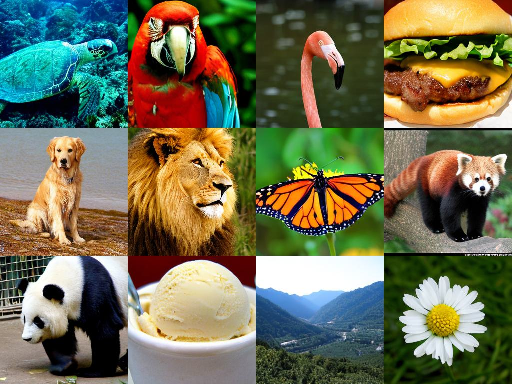
\includegraphics[width=\columnwidth]{plots/generation_samples.pdf}
    \caption{\textbf{\textit{Generated samples}} from our DiT-XL/2 model with Spiral RoPE trained for 7M steps on ImageNet $256 \times 256$. Images are generated using classifier-free guidance with scale 4.0.}
    \label{fig:generation_samples}
\end{figure}
